\usetikzlibrary{shapes.geometric}

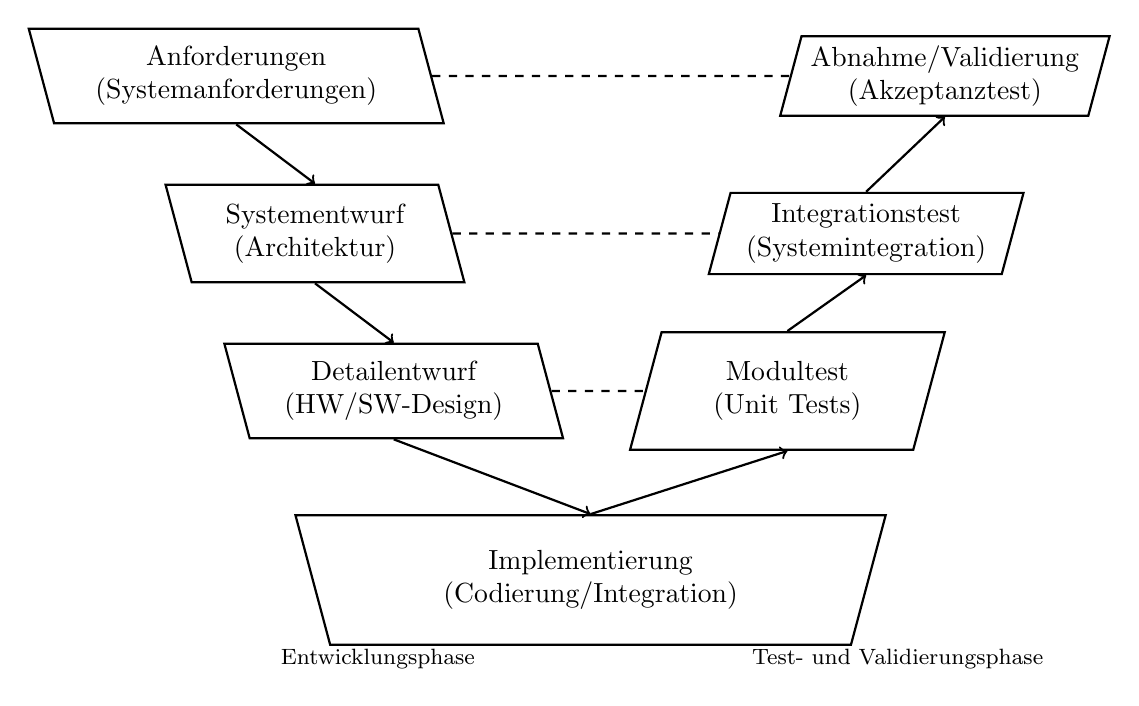
\begin{tikzpicture}[
	thick,
	boxleft/.style={
		draw, trapezium,
		trapezium left angle=105,
		trapezium right angle=75,
		align=center,
		minimum width=3.8cm,
		minimum height=1.2cm
	},
	box/.style={
		draw, trapezium,
		trapezium left angle=105,
		trapezium right angle=105,
		align=center,
		minimum width=7.5cm,
		minimum height=0.95cm
	},
	boxright/.style={
		draw, trapezium,
		trapezium left angle=75,
		trapezium right angle=105,
		align=center,
		minimum width=4cm,
		minimum height=0.95cm
	}
	]
	
	\node[boxleft] (req)  at (0,8)  {Anforderungen\\(Systemanforderungen)};
	\node[boxleft] (sys)  at (1,6) {Systementwurf\\(Architektur)};
	\node[boxleft] (sw)   at (2,4) {Detailentwurf\\(HW/SW-Design)};
	\node[box]     (impl) at (4.5,1.6) {Implementierung\\(Codierung/Integration)};
	
	\node[boxright] (unit) at (7,4) {Modultest\\(Unit Tests)    };%\\(Unit Test)};
	\node[boxright] (int)  at (8,6) {Integrationstest\\(Systemintegration)};
	\node[boxright] (acc)  at (9,8) {Abnahme/Validierung\\(Akzeptanztest)};
	
	\draw[->] (req.south) -- (sys.north);
	\draw[->] (sys.south) -- (sw.north);
	\draw[->] (sw.south)  -- (impl.north);
	
	\draw[->] (impl.north) -- (unit.south);
	
	\draw[->] (unit.north) -- (int.south);
	\draw[->] (int.north)  -- (acc.south);
	
	\draw[dashed] (sw.east)  -- (unit.west);
	\draw[dashed] (sys.east) -- (int.west);
	\draw[dashed] (req.east) -- (acc.west);
	
	\node[align=center] at (1.8,0.6) {\footnotesize Entwicklungsphase};
	\node[align=center] at (8.4,0.6) {\footnotesize Test- und Validierungsphase};
	
\end{tikzpicture}
